\documentclass[12pt, twocolumn]{article}
\usepackage[utf8]{inputenc}
\usepackage[spanish]{babel}
\usepackage{geometry}
\geometry{a4paper,margin=0.8in}
\usepackage{amsmath}
\usepackage{listings}
\usepackage{graphicx}
\usepackage{float}
\usepackage{url}
\usepackage{booktabs}
\usepackage{chngcntr}
\usepackage{amsfonts}
\usepackage{fancyhdr}
\pagestyle{fancy}
\cfoot{Página \thepage}
\counterwithin*{equation}{subsection}

\begin{document}
	\title{Generalización de Terrenos con Redes Neuronales Multicapa \\ 
		   \large{\textsc{Sistemas de Inteligencia Artificial}} \\
		   \normalsize{\textsc{Instituto Tecnológico de Buenos Aires}}}
	\author{
		\textsc{Garrigó}, Mariano \\
		\texttt{54393}
		\and
		\textsc{Raies}, Tomás A. \\
		\texttt{56099}
		\and
		\textsc{Saqués}, M. Alejo \\
		\texttt{56047} 
	}
	\date{}
	\maketitle
	
	\begin{abstract}
		Se ha analizado el potencial de una red neuronal multicapa supervisada a los efectos de aprender la forma de un terreno, y, posteriormente, generalizar sobre la misma.
		
		Se ha evaluado una serie de variaciones sobre el algoritmo de \textit{backpropagation}, particularmente \textit{adaptive eta} y \textit{momentum}, como así también combinaciones de ambas técnicas. Asimismo, se han comparado los resultados obtenidos actualizando los pesos de la red tanto de manera incremental como en \textit{batch}. 
		
		Asimismo, se han entrenado diversas redes con capacidad de generalizar terrenos de diferentes ciudades del mundo, tomando como referencia puntos tomados de mapas de altura de dichas ciudades.
		
		Por último, se han comparado estas técnicas con el estado del arte en algoritmos de generación aleatoria de terrenos, como el \textit{Diamond-Square Algorithm} (DSA). El objetivo ha sido probar las capacidades de una red neuronal de aprender terrenos con una \textit{apariencia} lo más aleatoria posible, tal como busca lograr DSA. 
	\end{abstract}
	
	\paragraph{Palabras clave:} Redes multicapa supervisadas, \textit{feature scaling}, \textit{backpropagation}, \textit{adaptive eta}, \textit{momentum}, actualización de pesos incremental / en \textit{batch}, funciones de activación, \textit{Diamond-Square Algorithm}.
	
	\section{Descripción del entrenamiento}
	
	\paragraph{} En esta sección, se discutirán las decisiones tomadas por el Equipo para entrenar redes neuronales. Esto incluye tanto toda la instancia de pre-procesamiento, como así también el entrenamiento propiamente dicho. 
	
	\subsection{Pre-procesamiento}
	
	\subsubsection{\textit{Feature scaling}}
	
	\paragraph{} Dado que las imágenes de las funciones de activación son intervalos en $\mathbb{R}^{2}$ ($tanh : \mathbb{R} \to \left[-1, 1\right]$ y $logistic : \mathbb{R} \to \left[0, 1\right]$), si los datos del \textit{set} de entrenamiento no se encuentran dentro de dichos intervalos, cierto ajuste es necesario.
	
	\paragraph{} Para ello, se utiliza \textit{feature scaling} para estandarizar muestras en algún intervalo deseado. De todas las variaciones de dicho método, se utiliza el \textit{rescaling} de datos:
	
	\begin{align}
		x_{i}^{'} = \frac{x_{i}-min(X)}{max(X)-min(X)}(b-a)+a
	\end{align}
	
	\paragraph{} Donde $X$ es el espacio de muestras a estandarizar, $a$ y $b$ son las cotas inferior y superior del intervalo de llegada, respectivamente. 
	
	\subsubsection{Selección de muestras de entrenamiento}
	
	\paragraph{} Dado que una de las características que se quiere probar es la capacidad de generalización de la red, es razonable que parte de las muestras del terreno se utilicen para verificar que la red, efectivamente, aprendió el problema. Por ende, se ha decidido utilizar el $90\%$ de las muestras para el entrenamiento, y un $10\%$ para testeo. Los patrones de cada conjunto se toman de manera no determinística. Se debe notar que la proporción es un dato parametrizable. 
	
	\subsection{Implementaciones de \textit{backpropagation}}
	
	\paragraph{} A continuación, se elaborará sobre los diferentes algoritmos utilizados para entrenar las redes neuronales. Las descripciones atacarán fundamentalmente aquellos rasgos distintivos de los mismos, que emanan de decisiones tomadas por el Equipo durante el proceso de desarrollo.
	
	\paragraph{Nota:} El error cuadrático medio sobre el conjunto de datos de entrenamiento se calcula, para cada versión del algoritmo, después de ejecutar cada \textit{epoch}.
	
	\subsubsection{Algoritmo incremental con \textit{adaptive eta} y \textit{momentum}}
	
	\paragraph{} Tal como su nombre lo indica, las actualizaciones de pesos en este algoritmo se realizan patrón a patrón. Esto lleva consigo la necesidad de iterar sobre todos los patrones en cada \textit{epoch}, desaprovechándose así las mejoras que realiza \textit{Octave/Matlab} sobre el producto matricial. Esto se verá reflejado en la lentitud de ejecución de cada \textit{epoch} por parte de este algoritmo, relativa a la versión en \textit{batch} que se mencionará a continuación.
	
	\paragraph{} En lo que respecta al orden de las muestras de entrenamiento en cada \textit{epoch}, se ha tomado la decisión de presentarlas en un orden no determinístico, dado que se ha observado que, de esta forma, es menos probable que el algoritmo se atasque en mínimos locales. 
	
	\paragraph{} Por último, se han considerado dos variaciones sobre el proceso de eta adaptativo, las cuales versan sobre si después de $k$ iteraciones en las que el error cuadrático medio descendió consistentemente, dicho contador se restablece tras incrementar el eta o si se prosigue incrementando \textit{epoch} tras \textit{epoch} hasta que haya un incremento en el error. Se ha notado que ambas variaciones presentan comportamientos similares si para la primera versión se establecen valores de $k$ \textit{pequeños} y, para la segunda versión, \textit{grandes}. Para el caso, \textit{pequeños} y \textit{grandes} valores se refieren a cifras en el orden de $10^{1}$ y $10^{2}$ respectivamente. Se ha decidido utilizar la versión que restablece $k$ tras cada incremento.
	
	\paragraph{} En lo que respecta a las condiciones de corte, el algoritmo retorna cuando:
	
	\begin{enumerate}
		\item Se ha llegado al máximo de iteraciones,
		\item Se ha llegado al valor del error cuadrático medio deseado,
		\item El eta se ha hecho $\sim 0$. 
		\item La diferencia entre el error cuadrático medio anterior y el actual es $0$.
	\end{enumerate}
	
	\paragraph{Nota:} El ítem $3.$ refleja la situación en la que el error ha crecido consistentemente, haciendo que tras sucesivas disminuciones del eta dicho valor se acerque a $0$. 
	
	
	\subsubsection{Algoritmo en \textit{batch} con \textit{momentum}}
	
	\paragraph{} En este algoritmo, las actualizaciones de pesos se realizan tras cada \textit{epoch}. A diferencia del caso anterior, esto permite tomar las muestras del set de entrenamiento de manera conjunta, sin tener que iterar por cada patrón. De esta forma, se aprovechan las mejoras que \textit{Octave/Matlab} realizan sobre el producto matricial, haciendo que la ejecución de cada \textit{epoch} sea notoriamente más rápida que en el algoritmo anterior. 
	
	\paragraph{} En lo que respecta a las condiciones de corte, el algoritmo retorna cuando:
	
	\begin{enumerate}
		\item Se ha llegado al máximo de iteraciones,
		\item Se ha llegado al valor del error cuadrático medio deseado,
		\item La diferencia entre el error cuadrático medio anterior y el actual es $\sim 0$.
	\end{enumerate}
	
	\subsubsection{Algoritmo en \textit{batches} de tamaño parametrizable}
	
	\paragraph{} La idea de esta versión de \textit{batch} es idéntica a la anterior, salvo que los \textit{batches} se toman de a tamaños parametrizables. Esta implementación busca aprovechar las mejoras en eficiencia del producto de matrices de menores dimensiones. 
	
	\newpage
	
	\section{Resultados del entrenamiento}
	
	\paragraph{} En esta sección, se discutirán los mejores resultados logrados con ambos algoritmos, exhibiéndose la progresión del error y analizándose la precisión de la red obtenida al generalizar el terreno.
	
	\paragraph{Glosario de terminología:}
	
	\begin{itemize}
		\item $f$: Función de activación
		\item $H$: Capas ocultas (\verb|array|)
		\item $\eta$: \textit{Learning rate}
		\item $momentum$: factor del \textit{momentum}
		\item $\alpha$: constante de crecimiento del eta adaptativo
		\item $\beta$: factor de decrecimiento del eta adaptativo
		\item $k$: constante de decrecimiento consistente
		\item $\epsilon$: cota inferior para $\eta$ (condición de corte)
		\item $\epsilon_{e}$: condición de corte del error cuadrático medio
		\item $max_{iters}$: número máximo de \textit{epochs}.
		
	\end{itemize}
	
	\subsection{Algoritmo incremental con \textit{adaptive eta}}
	
	\paragraph{} A continuación siguen los resultados obtenidos para el entrenamiento con el algoritmo incremental utilizando eta adaptativo.  
	
	\subsubsection{Parámetros y resultados generales} 
	
	\begin{itemize}
		\item $f = \tanh$
		\item $H = \left[10, 10\right]$
		\item $\eta = 0.1$
		\item $momentum = 0$
		\item $\alpha = 0.05$
		\item $\beta = 0.1$
		\item $k = 5$
		\item $\epsilon = 0.00001$
		\item $\epsilon_{e} = .0001$
		\item $max_{iters} = 10000$
	\end{itemize}
	
	\paragraph{} En este primer caso de análisis, se ha logrado obtener una red neuronal que aproxima el terreno con un error cuadrático medio sobre el \textit{set} de entrenamiento de $6.5*10^{-4}$. Es decir, la ejecución del algoritmo finalizó por haberse alcanzado el máximo de iteraciones. El \textit{set} de pesos que menor error cuadrático medio logró se correspondió con la iteración $9954$.
	
	\paragraph{} Un aspecto a destacar es la elección de no utilizar \textit{momentum}. Por lo general, al combinar \textit{momentum} con \textit{adaptive eta}, se ha encontrado que el comportamiento del error a lo largo del tiempo es mucho más errático que sin utilizar el primero. Por ende, se ha optado por no usar \textit{momentum} en este caso, optándose por usarlo como mecanismo de aceleración de \textit{backpropagation} en el algoritmo por \textit{batch}.
	
	\subsubsection{Tasas de éxito}
	
	\paragraph{} Un indicador de qué tan acertado fue el entrenamiento de la red se puede encontrar en las tasas de éxito, es decir, en qué proporción la red neuronal generalizó correctamente un nuevo dato. Para ello, se está tomando como punto de comparación el \textit{set} de muestras de prueba extraído tal como se indicó más arriba. Este conjunto representa el $10\%$ del conjunto original. Los intervalos dentro de los cuales se considera que el valor fue correctamente generalizado están definidos por el Épsilon ($\epsilon$): $\left[S_{i}-\epsilon, S_{i}+\epsilon\right]$.  
	
	\begin{table}[H]
		\centering
		\begin{tabular}{ll}
			\hline
			Épsilon & Éxito ($\%$)\\ \hline
			.05     & 75.6  \\
			.06     & 80    \\
			.07     & 84.5  \\
			.08     & 91.2  \\
			.09     & 91.2  \\
			.1      & 97.8  \\
			.11     & 100   \\ \hline
			\end{tabular}
			\caption{Tasas de éxito}
			\label{ex1}
	\end{table}
	
	\paragraph{} Como se podrá ver, con valores relativamente pequeños del Épsilon se logra tasas altas de éxito, considerando que el espacio de llegada (la coordenada $Z$) toma valores en el intervalo $\left[-1, 1\right]$.
	
	\subsubsection{Errores cometidos en el \text{set} de comparación}
	
	\paragraph{} En estrecha vinculación con el punto anterior, se puede analizar la diferencia entre el valor esperado y el valor emitido por la red. Esto está definido por:
	
	\begin{align}
		D_{i} = abs(S_{c_{i}}-E_{i})
	\end{align}
	
	\paragraph{} Donde $E_{i}$ es la evaluación del i-ésimo patrón, $S_{c_{i}}$ es su salida esperada.
	
	\paragraph{} Este análisis arroja los siguientes resultados:
	
	\begin{itemize}
		\item $max(D) = 0.10006$
		\item $min(D) = 1.7035*10^{-4}$
		\item $mean(D) = 0.030684$
	\end{itemize}
	
	\paragraph{} Cómo se puede ver, los valores están en línea con los resultados de la sección anterior. El valor más significativo en este punto es la media de las diferencias, que, como podrá observarse, es pequeña en relación a la longitud del espacio de llegada. 
	
	\paragraph{} A continuación se presenta la gráfica de cada una de las diferencias entre los valores esperado y calculado.
	
	\begin{figure}[H]
		\centering
		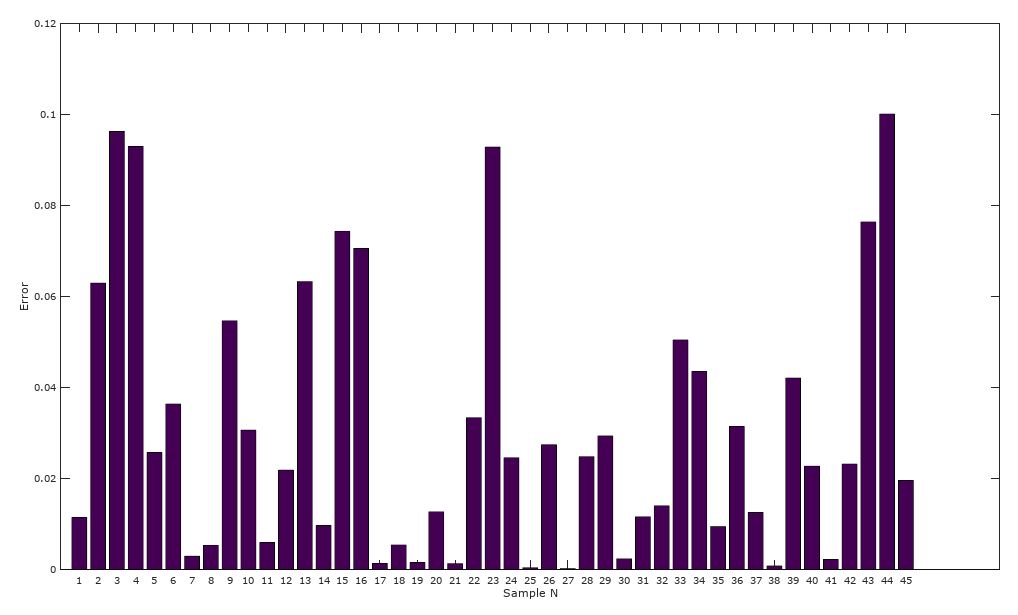
\includegraphics[width=8.5cm]{../results/adaptive_eta_incremental/3/bar_incremental.png}
		\caption{$D_i$}
		\label{di1}
	\end{figure}
	
	\paragraph{} Como puede verse en la figura \ref{di1}, existen picos en los cuales la diferencia es mucho mayor a la del resto. Analizar a qué puntos corresponden dichos valores permitirá comprender el comportamiento de la red.
	
	\begin{table}[H]
		\centering
		\begin{tabular}{lll}
			\hline
			Muestra & \multicolumn{1}{c}{X} & \multicolumn{1}{c}{Y} \\ \hline
			44      & -0.14806              & 0.31066               \\
			3       & -1                    & -0.93007              \\
			23      & 1                     & -0.11425              \\
			4       & 0.061232              & -0.240449             \\ \hline
		\end{tabular}
		\caption{Puntos de mayor $D_{i}$}
		\label{p1}
	\end{table}
	
	\paragraph{} En la tabla \ref{p1} se pueden observar algunos datos interesantes. Las muestras $3$ y $23$ se localizan aproximadamente en dos diferentes puntas del terreno. Esto podría estar indicando que la red neuronal tiene mayores dificultades en aprender las puntas por ciertas características particulares que las mismas podrían tener.
	
	\begin{figure}[H]
		\centering
		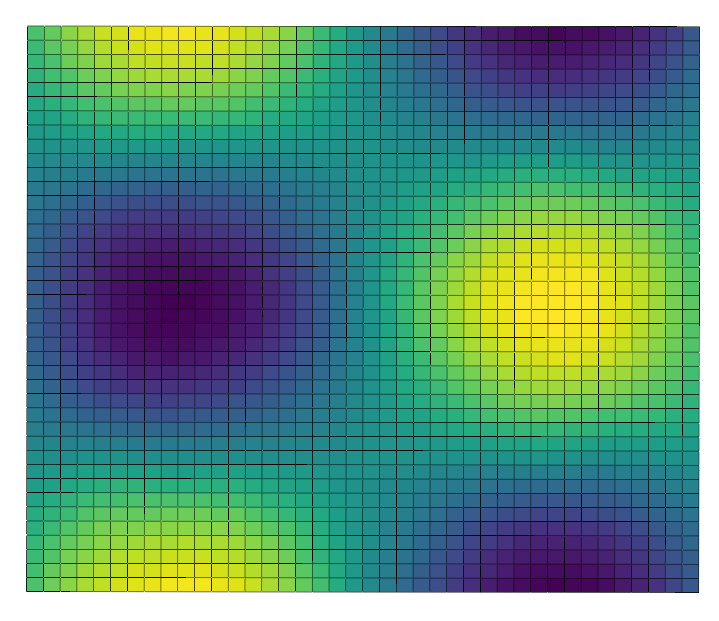
\includegraphics[width=8cm]{../results/heightmap.png}
		\caption{Mapa de altura}
		\label{heightmap}
	\end{figure}
	
	\paragraph{} Como se podrá ver en el mapa de altura de la figura \ref{heightmap}, realizado mediante una generalización realizada por la red, en las puntas hay o bien depresiones muy acentuadas o elevaciones pronunciadas. Nótese que colores mas azulados reflejan puntos más bajos. 
	
	\paragraph{} Observando los valores de la muestra 4, puede afirmarse que este se encuentra en las inmediaciones de uno de los extremos del terreno, por lo que es de esperar que el comportamiento sea similar al de los casos anteriores.
	
	\subsubsection{Análisis del error cuadrático medio}
	
	\paragraph{} Para analizar la evolución del error cuadrático medio en el tiempo, la gráfica a continuación puede ayudar a entender su comportamiento. 
	
	\begin{figure}[H]
		\centering
		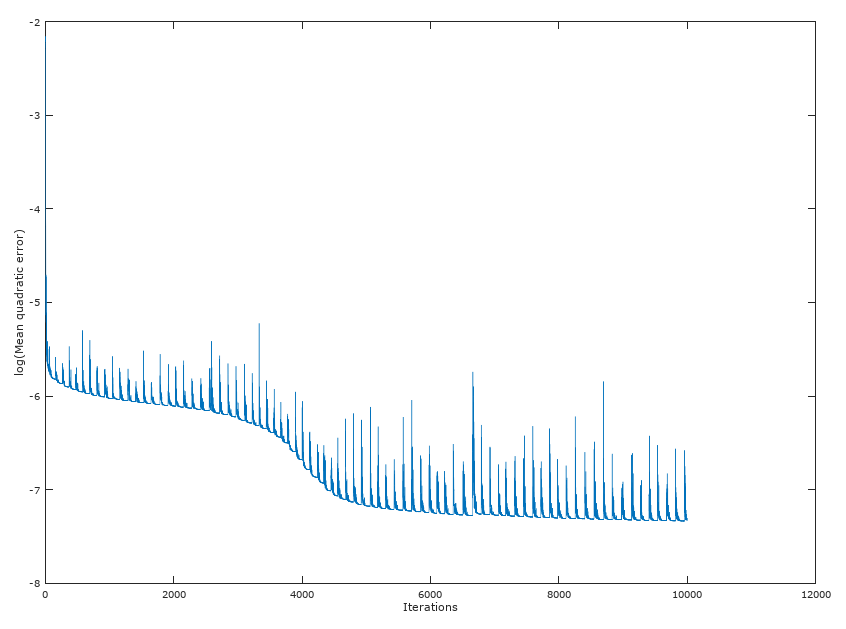
\includegraphics[width=9cm]{../results/adaptive_eta_incremental/3/log_incremental.png}
		\caption{Error cuadrático medio}
		\label{error1}
	\end{figure}
	
	\paragraph{} La figura \ref{error1} es una gráfica en escala logarítmica del error cuadrático medio en función del número de iteración. El aspecto quizás más interesante que se puede observar es la periodicidad con la que el error muestra picos de aumento, rápidamente corrigiéndose para mostrar el error una tendencia decreciente. Dicha periodicidad está relacionada con el valor $k$, es decir, el número de \textit{epochs} que se considera que expresa un decrecimiento consistente en el error. Es probable que lo que se observe sea que, al aumentar el eta, el error inicialmente aumenta para luego corregirse.
	
	\paragraph{} Otro aspecto interesante es el abrupto descenso del error en torno a la iteración 4000, sobre todo teniendo en cuenta que la pendiente de la curva, hasta ese momento, era similar a lo que se encuentra en torno a la iteración 6000, es decir, después de dicho suceso. Queda como interrogante el analizar si un descenso como tal podría haber ocurrido de haberse proseguido la ejecución. De todas formas, se considera que el error alcanzado resuelve con creces el objetivo del problema con errores mínimos, tal como se ha discutido en secciones anteriores. 

	
	\subsection{Algoritmo en \textit{batch} con \textit{momentum}}
	
	\paragraph{} En este apartado se discutirán los resultados obtenidos al entrenar la red neuronal realizando las actualizaciones de pesos en \textit{batch}.
	
	\subsubsection{Parámetros y resultados generales} 
	
	\begin{itemize}
		\item $f = \tanh$
		\item $H = \left[10, 10\right]$
		\item $\eta = 0.001$
		\item $momentum = .9$
		\item $\epsilon_{e} = .0001$
		\item $max_{iters} = 100000$
	\end{itemize}
	
	\paragraph{} Si se compara el \textit{set} de parámetros iniciales con el del caso anterior, se podrá notar que el $\eta$ es considerablemente más pequeño. Esta decisión se puede asociar con el factor de que, a valores de $\eta$ \textit{grandes} (mayores a $10^{-2}$), el algoritmo tiende a atascarse en mínimos locales. 
	
	\paragraph{} Este último comentario está estrechamente vinculado con la decisión de utilizar \textit{momentum}. Dado que \textit{momentum} busca acelerar el proceso de entrenamiento adicionando una proporción de $\Delta W_{prev}$ (en particular, $0.9$), valores de $\eta$ relativamente \textit{grandes} pueden hacer desviar al algoritmo del camino correcto, así atascándose en mínimos locales o, incluso, aumentando el error indefinidamente $-$esto último se ha notado en algunos casos utilizando \textit{momentum} en el algoritmo incremental con \textit{adaptive eta}. Visto esto, se puede decir que la decisión tomada con respecto a los valores iniciales, además de $-$ como se verá $-$ funcionar en la práctica, tiene sus fundamentos teóricos.  
	
	\paragraph{} Con respecto a los resultados de la ejecución, se ha obtenido un error cuadrático medio sobre el conjunto de datos de entrenamiento de $3.26*10^{-4}$, es decir, prácticamente la mitad del error obtenido en el caso anterior. Sin embargo, es de notar que dicho valor fue conseguido en $100000$ \textit{epochs}, lo cual supuso un tiempo de entrenamiento de $01:15$ horas en una computadora con un procesador \textbf{Intel Core i7-4700MQ}. Este tiempo supera con creces al del caso anterior, que no superó la media hora. El análisis de la generalización de esta red ayudará a discernir entre qué red presenta una mejor relación resultados/esfuerzo computacional. 
	
	\subsubsection{Tasas de éxito}
	
	\paragraph{} Al igual que el caso anterior, se buscará analizar dentro de qué intervalos la red obtenida generaliza correctamente datos de prueba, es decir, no vistos durante el entrenamiento. 
	
	\begin{table}[H]
		\centering
		\begin{tabular}{ll}
			\hline
			Épsilon & Éxito ($\%$)\\ \hline
			.05     & 88.9  \\
			.06     & 93.4    \\
			.07     & 95.6  \\
			.08     & 97.8  \\
			.09     & 100  \\
			.1      & 100  \\ \hline
		\end{tabular}
		\caption{Tasas de éxito}
		\label{ex2}
	\end{table}
	
	\paragraph{} Como podrá verse, a diferencia del caso anterior, todas las muestras de prueba son generalizadas correctamente en un intervalo de $\pm 0.1$, teniendo entorno a un $89\%$ de éxito incluso con intervalos el doble de pequeños. Analizando el último caso mencionado, este valor es alrededor de un $14\%$ mejor que su equivalente en los resultados del algoritmo anterior. 
	
	\subsubsection{Errores cometidos en el \text{set} de comparación}
	
	\paragraph{} Algunas de las cifras que describen a los resultados del \textit{set} de comparación son las siguientes:
	
	\begin{itemize}
		\item $max(D) = 0.085488$
		\item $min(D) = 9.3254*10^{-4}$
		\item $mean(D) = 0.021261$
	\end{itemize}
	
	\paragraph{} El valor que más dista del obtenido en la ejecución anterior es el $min(D)$, que se aproxima a ser 1 orden de magnitud inferior a su equivalente del caso anterior. Por lo demás, los otros valores son, razonablemente inferiores, siendo la media de la diferencia entre los valores esperado y calculado inferior entorno a $\frac{1}{3}$. 
	
	\paragraph{} El siguiente gráfico muestra los errores de cada coordenada:
	
	\begin{figure}[H]
		\centering
		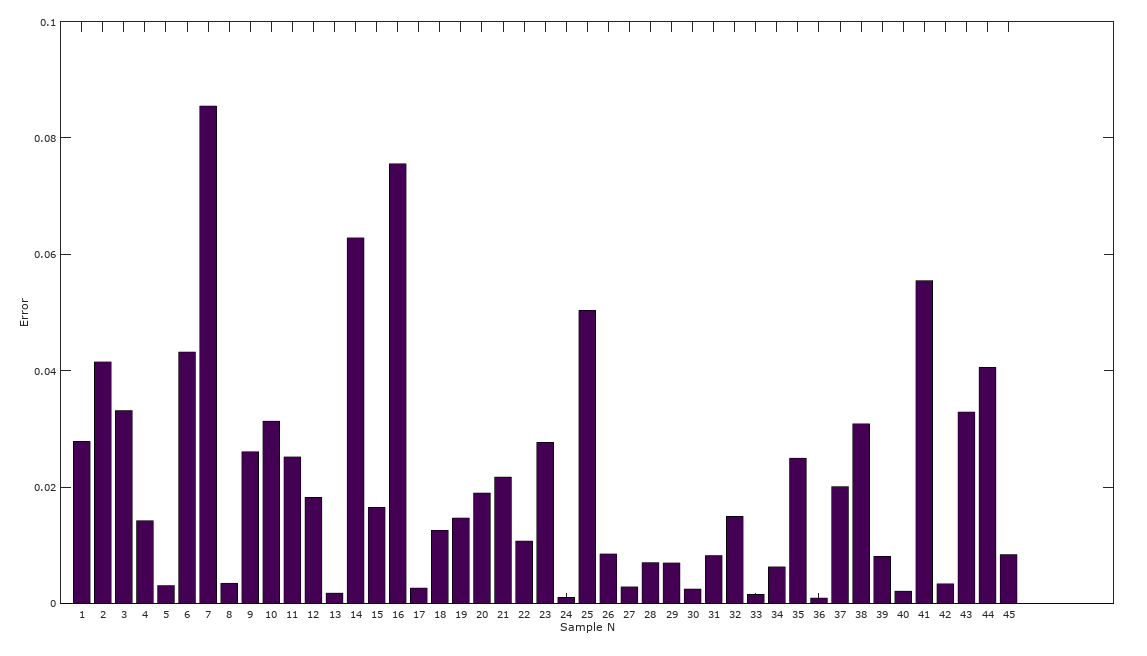
\includegraphics[width=8.5cm]{../results/batch_momentum/2/bar_batch.png}
		\caption{$D_i$}
		\label{di2}
	\end{figure}
	
	\paragraph{} Mediante una simple inspección de la gráfica en \ref{di2}, comparándola con su equivalente anterior (\ref{di1}), se puede percibir que la cantidad de \textit{picos} $-$ barras cuya longitud es más del doble que el resto $-$ no solamente es inferior, sino que son de menor magnitud. 
	
	\paragraph{} De todas formas, se procederá a realizar el mismo análisis con respecto a la ubicación de los puntos con generalización más deficiente:
	
	
	\begin{table}[H]
		\centering
		\begin{tabular}{lll}
			\hline
			Muestra & \multicolumn{1}{c}{X} & \multicolumn{1}{c}{Y} \\ \hline
			7      & 1             & 0.58233             \\
			16       & 1                    & 0.82133              \\
			14      & -0.14806                     & -0.35267              \\
			41       & 0.94275              & -0.24045             \\ \hline
		\end{tabular}
		\caption{Puntos de mayor $D_{i}$}
		\label{p2}
	\end{table}
	
	\paragraph{} Como podrá notarse en el cuadro \ref{p2}, las conclusiones que se pueden extraer son similares a las encontradas en (\ref{p1}). Las muestras $16$ y $41$ se encuentra aproximadamente en dos diferentes puntas, el caso $7$ sobre la mitad de un borde, y el caso $14$ en alguna región de alto gradiente. La conclusión que se puede extraer a propósito de esto es que más puntos pueden ser necesarios en estas regiones si se precisa un muy buen nivel de detalle, y que las dificultades son independientes de los algoritmos utilizados. Esto no quita que no exista una estructura de red neuronal que tenga un mejor potencial para aprender dichas regiones, pero se afirma que, de las decenas de configuraciones probadas, la que se presenta es la que mejores resultados ha exhibido. 
	
	\subsubsection{Análisis del error cuadrático medio}
	
	\paragraph{} Para concluir el análisis de los resultados para esta ejecución, a continuación se discutirá el comportamiento del error cuadrático medio en función del tiempo. 
	
	\begin{figure}[H]
		\centering
		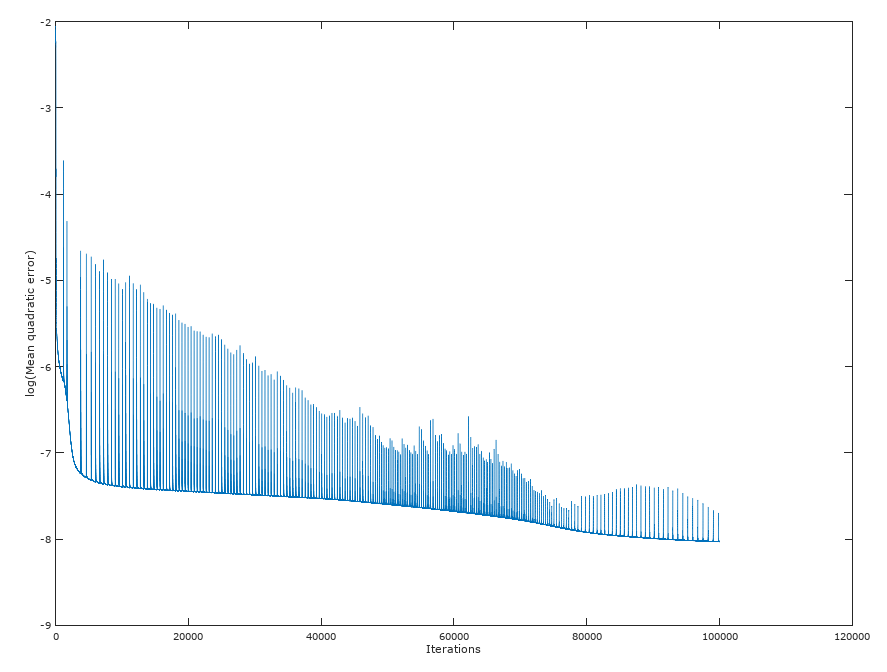
\includegraphics[width=9cm]{../results/batch_momentum/2/log_batch.png}
		\caption{Error cuadrático medio}
		\label{error2}
	\end{figure}
	
	\paragraph{} Lo que sin lugar a dudas impacta al observar esta gráfica es la periodicidad en con la que ocurren picos muy significativos en el error. Sin embargo, es de notar que la magnitud de dichos saltos tiende a decrecer en el tiempo, para lograr que el error tenga una tendencia generalmente decreciente. 
	
	\paragraph{} Se puede observar que, dentro de las primeras $20000$ iteraciones, los errores oscilan entre valores de $9*10^{-4}$ ($\exp(-7)$) y $6.7*10^{-3}$ ($\exp(-5)$), lo cual representa saltos de 1 orden de magnitud. 
	
	\paragraph{} Por último, puede notarse como hacia la iteración 80000 hubo un marcado incremento en la tasa de decrecimiento del error cuadrático medio, para luego asentarse en niveles comparados a los anteriores. 
	
	
	
	
	
	
	
	
\end{document}